% Pengaturan ukuran teks dan jenis dokumen
\documentclass[12pt]{article}

% Pengaturan ukuran halaman dan margin
\usepackage[a4paper,top=30mm,left=30mm,right=20mm,bottom=25mm]{geometry}

% Pengaturan ukuran spasi
\usepackage[singlespacing]{setspace}

% Judul dokumen
\title{Proposal Tugas Akhir ITS}
\author{Abdul Azis}

% Pengaturan format bahasa
\usepackage[indonesian]{babel}

% Pengaturan detail pada file PDF
\usepackage[pdfauthor={\@author},bookmarksnumbered,pdfborder={0 0 0}]{hyperref}

% Pengaturan jenis karakter
\usepackage[utf8]{inputenc}

% Package lainnya
\usepackage[skip=10pt plus1pt, indent=2em]{parskip}
\usepackage{chngcntr}
\usepackage{mathptmx}
\usepackage{times}
\usepackage{etoolbox} % Mengubah fungsi default
\usepackage{enumitem} % Pembuatan list
\usepackage{lipsum} % Pembuatan template kalimat
\usepackage{graphicx} % Input gambar
\usepackage{longtable} % Pembuatan tabel
\usepackage[table,xcdraw]{xcolor} % Pewarnaan tabel
\usepackage[numbers]{natbib} % Kutipan artikel
\usepackage{changepage} % Pembuatan teks kolom
\usepackage{multicol} % Pembuatan kolom ganda
\usepackage{multirow} % Pembuatan baris ganda

% Pengaturan format judul bab
\usepackage{titlesec}
\renewcommand{\thesection}{\arabic{section}}
\titleformat*{\section}{\large\bfseries}
\titleformat*{\subsection}{\large\bfseries}
\titlespacing{\section}{0ex}{3ex}{1.5ex}
\titlespacing{\subsection}{0ex}{3ex}{1.5ex}

% Isi keseluruhan dokumen
\begin{document}

% % Menonaktifkan penomoran halaman
% \pagenumbering{gobble}

% Lembar pengesahan
% \begin{flushleft}
  % Ubah kalimat berikut sesuai dengan nama departemen dan fakultas
  \textbf{Departemen Teknik Komputer - FTEIC}\\
  \textbf{Institut Teknologi Sepuluh Nopember}\\
\end{flushleft}

\begin{center}
  % Ubah detail mata kuliah berikut sesuai dengan yang ditentukan oleh departemen
  \underline{\textbf{EC224701 - PRA TUGAS AKHIR - 2 SKS}}
\end{center}

\begin{adjustwidth}{-0.2cm}{}
  \begin{tabular}{lcp{0.7\linewidth}}

    % Ubah kalimat-kalimat berikut sesuai dengan nama dan NRP mahasiswa
    Nama Mahasiswa     & : & Abdul Azis                                                          \\
    Nomor Pokok        & : & 0721 19 4000 7004                                                   \\

    % Ubah kalimat berikut sesuai dengan semester pengajuan proposal
    Semester           & : & Ganjil 2022/2023                                                    \\

    % Ubah kalimat-kalimat berikut sesuai dengan nama-nama dosen pembimbing
    Dosen Pembimbing   & : & 1. Dr. Supeno Mardi Susiki Nugroho, S.T, M.T.                       \\
                       &   & 2. Reza Fuad Rachmadi, S.T., M.T., Ph.D                             \\
    % Ubah kalimat berikut sesuai dengan judul tugas akhir
    Judul Tugas Akhir  & : & \textbf{Elective and Enrichment Course Recommender System}          \\
                       &   & \textbf{using Decision Tree On Learning, Management System Website} \\

    Uraian Tugas Akhir & : &                                                                     \\
  \end{tabular}
\end{adjustwidth}

Mahasiswa yang sedang menempuh semester empat atau selanjutnya biasanya akan merencanakan
untuk mengambil mata kuliah pilihan maupun mata kuliah penganyaan. Permasalahan yang biasanya dihadapi oleh mahasiswa
saat akan melakukan pengambilan mata kuliah adalah kebingungan dalam memilih mata kuliah
yang sesuai minat dan kemampuan mereka. Banyak mahasiswa yang masih belum memiliki gambaran
tentang minat pada mata kuliah disemester selanjutnya. Oleh karena itu, sistem rekomendasi
sangat cocok untuk dapat membantu mahasiswa dalam memutuskan mata kuliah apa yang akan mereka
untuk ditempuh disemester selanjutnya. Oleh karena itu dibutuhkan sebuah sistem yang dapat memberikan
rekomendasi mata kuliah kepada mahasiswa sehingga dapat membantu mahasiswa membuat keputusan saat akan
mengambil mata kuliah.
\vspace{1ex}

\begin{flushright}
  Surabaya, 23 Oktober 2022
\end{flushright}
\vspace{1ex}

\begin{center}

  \begin{multicols}{2}

    Dosen Pembimbing 1
    \vspace{12ex}

    % Ubah kalimat-kalimat berikut sesuai dengan nama dan NIP dosen pembimbing kedua
    \underline{Dr. Supeno Mardi Susiki Nugroho, S.T, M.T.} \\
    NIP. 19700313 199512 1 001

    \columnbreak

    Dosen Pembimbing 2
    \vspace{12ex}

    % Ubah kalimat-kalimat berikut sesuai dengan nama dan NIP dosen pembimbing kedua
    \underline{Reza Fuad Rachmadi, S.T., M.T., Ph.D} \\
    NIP. 19850403201212 1 000

  \end{multicols}

  % Dosen Pembimbing \\
  % \vspace{12ex}
  % % Ubah kalimat-kalimat berikut sesuai dengan nama dan NIP dosen pembimbing pertama
  % \underline{Dr. Supeno Mardi Susiki Nugroho, S.T, M.T.} \\
  % NIP. 19700313 199512 1 001

  \vspace{6ex}

  Mengetahui, \\
  % Ubah kalimat berikut sesuai dengan jabatan kepala departemen
  Kepala Departemen Teknik Komputerr FTEIC - ITS
  \vspace{12ex}

  % Ubah kalimat-kalimat berikut sesuai dengan nama dan NIP kepala departemen
  \underline{Dr. Supeno Mardi Susiki Nugroho, S.T, M.T.} \\
  NIP. 19700313 199512 1 001

\end{center}

\newpage

% Konten pendahuluan
\chapter{PENDAHULUAN}

\section{Latar Belakang}

Mahasiswa yang sedang menempuh semester empat atau selanjutnya biasanya akan merencanakan untuk mengambil
mata kuliah pilihan maupun mata kuliah penganyaan. Proses ini biasanya dilakukan diawal semester sebelum proses perkuliahan
dimulai untuk mengambil mata kuliah yang akan ditempuh disemester yang baru. Dalam suatu perguruan tinggi, mahasiswa belajar dalam suatu
sistem kurikulum yang terdiri atas sekumpulan daftar mata kuliah dimana setelah menempuh mata kuliah,
mahasiswa akan mendapatkan nilai. Nilai mata kuliah yang akan diterima didasarkan atas kemampuan
mahasiswa.

Permasalahan yang biasanya dihadapi oleh mahasiswa saat akan melakukan pengambilan mata kuliah adalah kebingungan dalam
memilih mata kuliah yang sesuai minat dan kemampuan mereka. Banyak mahasiswa yang masih belum memiliki gambaran tentang
minat pada mata kuliah disemester selanjutnya. Tak sedikit pula mahasiswa yang telah memiliki perminatan tetapi masih
bingung dalam memilih mata kuliah yang akan ditempuh. Hal ini biasanya terjadi karena kurangnya pemahaman mengenai
keterkaitan antar mata kuliah yang telah, sedang dan akan ditempuh. Oleh karena itu, sistem rekomendasi sangat cocok untuk
dapat membantu mahasiswa dalam memutuskan mata kuliah apa yang akan mereka untuk ditempuh disemester selanjutnya.

Sistem rekomendasi adalah sistem yang bertujuan untuk memberikan rekomendasi item yang menarik bagi pengguna agar pengguna
dapat memutuskan item apa yang akan mereka pilih. Belakangan ini, sistem rekomendasi telah menjadi sangat populer dan menjadi
sebuah bagian yang penting diberbagai layanan. Salah satu teknik yang dapat digunakan untuk mengatasi permasalahan tersebut adalah
penerapannya pada \emph{Deep Learning}.

\section{Rumusan Masalah}
Berdasarkan uraian latar belakang diatas dapat dirumuskan permasalahan sebagai berikut:
\begin{enumerate}[noitemsep]
      \item Bagaimana sistem rekomendasi dapat memberikan rekomendasi mata kuliah pilihan dan pengayaan
            yang cocok dengan mahasiswa?
      \item Bagaimana mengetahui kelayakan sistem rekomendasi yang dibangun dari pendekatan digunakan?
\end{enumerate}

\section{Batasan Masalah}
Batasan-batasan permasalahan yang dijadikan sebagai pedoman dalam pelaksanaan penelitian ini adalah sebagai berikut:
\begin{enumerate}[noitemsep]
      \item Sistem rekomendasi ini pemilihan mata kuliah ini hanya digunakan sebagai rekomendasi bagi mahasiswa, keputusan pemilihan mata kuliah ada kepada mahasiswa.
      \item Metode yang digunakan adalah \emph{Collaborative Filtering} dan \emph{Content-Based Filtering} dengan menggunakan metode \emph{Deep Learning}.
      \item Data latih yang digunakan berupa data mahasiswa, data mata kuliah, dan data nilai mahasiswa yang ada di Departemen Teknik Komputer ITS.
\end{enumerate}

\section{Tujuan Penelitian}
Tujuan penelitian ini dilakukan adalah:
\begin{enumerate}[noitemsep]
      \item Untuk merancang dan membuat sebuah sistem sehingga dapat memberikan rekomendasi mata kuliah pilihan
            maupun mata kuliah pengayaan yang mungkin cocok dengan mahasiswa.
      \item Untuk mengetahui kelayakan sistem rekomendasi yang dibangun pendekatan digunakan.
\end{enumerate}

\section{Manfaat}
Hasil penelitian ini yang diharapkan agar dapat memberikan manfaat sebagai berikut:
\begin{enumerate}[noitemsep]
      \item Bagi penulis yaitu untuk menambahkan pengetahuan dalam membangun sebuah sistem
            otomatisasi dengan menggunakan \emph{deep learning} berbasis Sistem Rekomendasi
            dengan pendekatan \emph{hybrid recommender system} menggunakan \emph{collaborative filtering} dan \emph{content-based filtering}.
      \item Memberikan manfaat bagi pengembangan ilmu pengetahuan dan teknologi serta wawasan ilmu bagi
            penelitian dan pengembangan selanjutnya.
      \item Memberikan kemudahan bagi mahasiswa agar dapat terbantu dengan adanya sistem yang dapat memberikan rekomendasi matakuliah yang mungkin cocok dengan preferensi mereka.
\end{enumerate}

% Konten tinjauan pustaka
\section{TINJAUAN PUSTAKA}

\subsection{Penelitian Terdahulu}

Penelitian mengenai rekomendasi mata kuliah telah di lakukan. Pada tahun 2019 Glenn Ferio, Rolly Intan, dan Silvia Rostianingsih melakukan
penelitian mengenai sistem rekomendasi mata kuliah pilihan pada \emph{paper} yang berjudul
\emph{Sistem Rekomendasi Mata Kuliah Pilihan Menggunakan Metode User Based Collaborative Filtering Berbasis Algoritma Adjusted Cosine Similarity}.
Input yang digunakan dalam penelitian ini adalah nilai-nilai mata kuliah yang didapatkan oleh mahasiswa. Pada penelitian ini mereka menggunakan algoritma
\emph{Cosine Similarity}, \emph{Adjusted Cosine Similarity}, dan model \emph{K-Nearest Neighbors}. Pada penelitian tersebut mereka mendapatkan akurasi
pada data \emph{testing} sebesar 69.24\% untuk algoritma \emph{Cosine Similarity} dan 83.55\% untuk algoritma \emph{Adjusted Cosine Similarity}.

\begin{table} [ht]
  \centering
  \counterwithin{table}{section}
  \caption{Hasil akurasi algoritma \emph{Cosine Similarity} dan \emph{Adjusted Cosine Similarity}}
  \vspace*{3mm}
  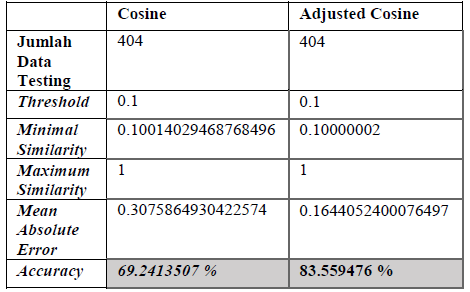
\includegraphics{gambar/akurasi-algoritma-cosine-similarity.png}
\end{table}

Dan mendapatkan akurasi pada data \emph{testing} menggunakan model \emph{K-Nearest Neighbors} dengan jumlah K = 16 sebesar 89.31\%
dan mendapatkan Mean Absolute Error sekitar 10.75.

\begin{figure} [ht]
  \centering
  \counterwithin{figure}{section}
  \caption{Visualisasi Mean Absolute Error model \emph{K-Nearest Neighbors}}
  \vspace*{3mm}
  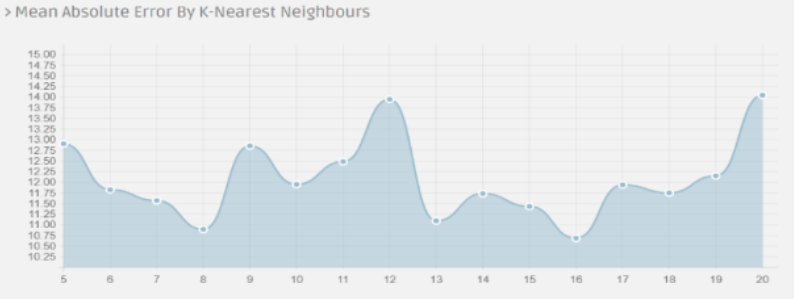
\includegraphics{gambar/mae-knn.png}
\end{figure}

Pada tahun 2022 Edward Fernando, Panca Mudjiraharjo, dan Muhammad Aswin melakukan penelitian untuk membuat sistem rekomendasi
dengan pendekatan \emph{Collacorative filtering} dan algoritma \emph{K-Means Clustering}. Dalam penelitian ini, sistem rekomendasi
berbasis collaborative filtering dibangun dengan empat metode, yaitu \emph{jaccard distance}, \emph{euclidean distance}, \emph{cosine similiarity}, dan \emph{pearson correlation}.
Dari pengimplementasian keempat metode tersebut, sistem mampu melakukan prediksi terkait konsentrasi prodi mahasiswa dan juga rekomendasi mata kuliah
yang dapat diambil pada semester selanjutnya. Dari implementasi awal, didapatkan hasil bahwa metode yang paling optimal hingga yang kurang optimal
secara berurutan adalah metode \emph{cosine similiarity}, \emph{euclidean distance}, \emph{jaccard distance}, lalu \emph{pearson correlatio}n.

\begin{table} [ht]
  \centering
  \counterwithin{table}{section}
  \caption{Nilai Kenaikan Akurasi Pendekatan \emph{Collaborative Filtering} dengan \emph{K-Means Clustering}}
  \vspace*{3mm}
  \begin{tabular}{|c|cc|c|}
    \hline
    \multirow{2}{*}{Metode} & \multicolumn{2}{c|}{\begin{tabular}[c]{@{}c@{}}Moving Average Akurasi \\ MK\end{tabular}} & \multirow{2}{*}{Kenaikan Akurasi}                                  \\ \cline{2-3}
                            & \multicolumn{1}{c|}{\begin{tabular}[c]{@{}c@{}}Sebelum \\ K-means\end{tabular}}           & \begin{tabular}[c]{@{}c@{}}Sesusah\\ K-Means\end{tabular} &        \\ \hline
    Jaccard                 & \multicolumn{1}{c|}{51.18\%}                                                              & 53.66\%                                                   & 4.83\% \\ \hline
    Euclidean Distance      & \multicolumn{1}{c|}{56.44\%}                                                              & 62.04\%                                                   & 9.92\% \\ \hline
    Cosine Similiarity      & \multicolumn{1}{c|}{59.25\%}                                                              & 64.76\%                                                   & 9.30\% \\ \hline
    Pearson Correlation     & \multicolumn{1}{c|}{40.83\%}                                                              & 43.71\%                                                   & 7.05\% \\ \hline
  \end{tabular}
\end{table}

Proses optimalisasi hasil rekomendasi mata kuliah pada penelitian ini dilakukan dengan melakukan seleksi rekomendasi berdasarkan tabel keputusan
yang dioleh menggunakan metode \emph{K-Means Clustering}. \emph{K-Means Clustering} mampu melakukan klasterisasi dari seluruh mata kuliah yang muncul dalam rekomendasi
dan memberikan label untuk mana mata kuliah yang direkomendasikan dan tidak direkomendasikan. Pada pengimplementasiannya, tabel keputusan \emph{K-Means Clustering}
mampu meningkatkan nilai akurasi \emph{moving average} pada setiap metode pendekatan \emph{collaborative filtering} dengan persentase peningkatan akurasi secara berurutan
dari yang paling optimal hingga kurang optimal yaitu \emph{euclidean distance} sebesar 9.92\%, \emph{cosine similiarity} sebesar 9.30\%, \emph{pearson correlation} sebesar 7.05\%,
dan \emph{jaccard} sebesar 4.83\%. Secara keseluruhan, sistem rekomendasi mata kuliah ini mampu melakukan prediksi konsentrasi mahasiswa hingga 84.78\% dan akurasi
\emph{moving average} pada prediksi rekomendasi mata kuliah hingga 64.76\% menggunakan data latih yang ditentukan. Dengan nilai \emph{mean absolute error} yang dihasilkan
pada penelitian ini, pendekatan \emph{collaborative filtering} yang paling optimal untuk perekomendasian mata kuliah jatuh pada metode \emph{cosine similiarity}.

\begin{table} [ht]
  \centering
  \counterwithin{table}{section}
  \caption{Nilai Mean Absolute Error Akurasi Mata Kuliah}
  \vspace*{3mm}
  \begin{tabular}{|c|cc|c|}
    \hline
    \multirow{2}{*}{Metode} & \multicolumn{2}{c|}{\begin{tabular}[c]{@{}c@{}}Moving Average Akurasi \\ MK\end{tabular}} & \multirow{2}{*}{Kenaikan Akurasi}                                  \\ \cline{2-3}
                            & \multicolumn{1}{c|}{\begin{tabular}[c]{@{}c@{}}Sebelum \\ K-means\end{tabular}}           & \begin{tabular}[c]{@{}c@{}}Sesusah\\ K-Means\end{tabular} &        \\ \hline
    Jaccard                 & \multicolumn{1}{c|}{51.18\%}                                                              & 53.66\%                                                   & 4.83\% \\ \hline
    Euclidean Distance      & \multicolumn{1}{c|}{56.44\%}                                                              & 62.04\%                                                   & 9.92\% \\ \hline
    Cosine Similiarity      & \multicolumn{1}{c|}{59.25\%}                                                              & 64.76\%                                                   & 9.30\% \\ \hline
    Pearson Correlation     & \multicolumn{1}{c|}{40.83\%}                                                              & 43.71\%                                                   & 7.05\% \\ \hline
  \end{tabular}
\end{table}

\subsection{Sistem Rekomendasi}





% Konten metodologi
\chapter{METODOLOGI}

\section{Metode yang digunakan}

Penelitian ini dilaksanakan sesuai dengan blok diagram pada Gambar 3.1. Blok diagram tersebut
merupakan metodologi penelitian yang disusun sesuai dengan langkah-langkah yang dilakukan dalam penelitian ini.

\begin{figure} [ht] \centering
  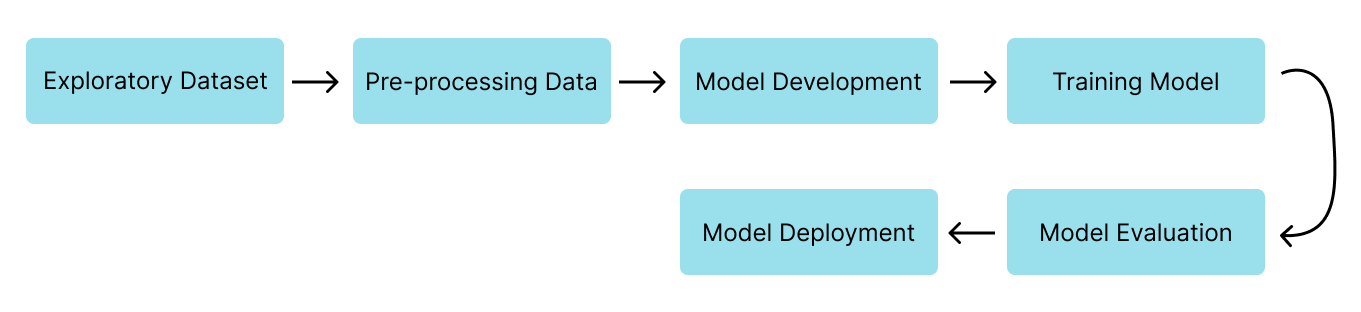
\includegraphics[width=160mm]{gambar/diagram-blok.png}
  \caption{Metodologi Penelitian}
\end{figure}

\section{Bahan dan peralatan yang digunakan}
\begin{enumerate}
  \item Komputer/Laptop
  \item Python
  \item Jupyter Notebook
  \item Tensorflow
  \item Docker
  \item Flask
\end{enumerate}

\section{Urutan pelaksanaan penelitian}

\begin{adjustwidth}{1em}{0pt}
  \addtocontents{toc}{\protect\setcounter{tocdepth}{1}}

  \subsection{Explorasi Dataset}
  Melakukan analisa pada data untuk mendapatkan gambaran awal pada data. Analisa yang dilakukan yaitu
  memeriksa informasi pada data (tipe data pada tiap data), memeriksa \emph{missing value} {(data yang hilang pada baris data)},
  memeriksa duplikasi pada data.

  \subsection{Pre-pemrosesan Data}
  Pada proses ini dataset yang telah dilakukan analisa akan dilakukan pra-pemrosesan sebelum dataset dapat digunakan
  untuk melakukan pelatihan pada model. Pada sistem rekomendasi pra-pemrosesan data yang biasa dilakukan seperti menghapus data
  yang tidak diperlukan untuk proses pelatihan, menghapus \emph{missing value} jika ada, melakukan normalisasi pada data (biasanya mentransformasikan data kedalam range yang sama),
  melakukan pembagian data pelatihan dan data percobaan.

  \subsection{\emph{Grades Prediction}}
  Untuk dapat menemukan mata kuliah yang mungkin sesuai dengan minat mahasiswa, diperlukan model yang dapat memprediksi nilai mata kuliah yang kemungkinan akan diambil oleh mahasiswa. Ini
  merupakan salah satu tahap dalam membangun sistem rekomendasi dengan pendekatan \emph{collaborative filtering} yang mana model akan memprediksi nilai yang akan didapatkan oleh mahasiswa dari berbagai mata kuliah
  yang belum pernah diambil sebelumnya oleh mahasiswa. Nilai yang diprediksi tidak hanya berdasarkan dari riwayat pengambilan mata kuliah dari satu orang mahasiswa, namun akan dilakukan pencocokan dengan mahasiwa
  lain yang memiliki preferensi yang saama. Setelah memprediksi nilai dari sekumpulan mata kuliah nantinya akan diambil \emph{top-N} mata kuliah dengan prediksi nilai tertinggi, setelah itu mata kuliah tersebut dapat direkomendasikan
  kepada mahasiswa.

  \subsection{\emph{Similarity Measure}}
  Tahap ini merupakan penerapan untuk pendekatan \emph{content-based filtering} yang mana model akan mencari kemiripan dari suatu mata kuliah, berdasarkan karakteristik yang dimiliki oleh mata kuliah tersebut.
  Setelah mendapatkan mendapatkan daftar mata kuliah yang mirip dengan input mata kuliah yang diberikan, hasil tersebut akan dikombinasikan dengan hasil rekomendasi dari model dengan pendekatan \emph{collaborative filtering}
  sehingga menghasilkan sistem rekomendasi dengan pendekatan \emph{hybrid recommender syste}.

  \subsection{Evaluasi Model}
  Evaluasi Model dilakukan dengan melakukan rekomendasi pada data percobaan. Jika dirasa rekomendasi belum cukup baik. Maka perlu melakukan \emph{tuning parameter} pada model seperti unit layer,
  jumlah layer pada model \emph{Deep Learning}, jumlah iterasi pelatihan dan beberapa parameter lain hingga model dapat memberikan rekomendasi dengan cukup baik.

  \subsection{\emph{Retrieval Recommendations}}
  Pada tahap ini model dari sistem rekomendasi yang telah dibuat sebelumnya ada dideploy atau dirilis agar dapat digunakan untuk memberikan rekomendasi melalui sebuah \emph{software}.
  \emph{Software} yang digunakan untuk menampilkan rekomendasi dari mata kuliah yang diberikan oleh model tersebut berupa website sederhana yang bisa menampilkan daftar mata kuliah
  yang direkomendasikan sesuai dengan ID/NRP dari mahasiswa.

  \begin{figure} [ht] \centering
    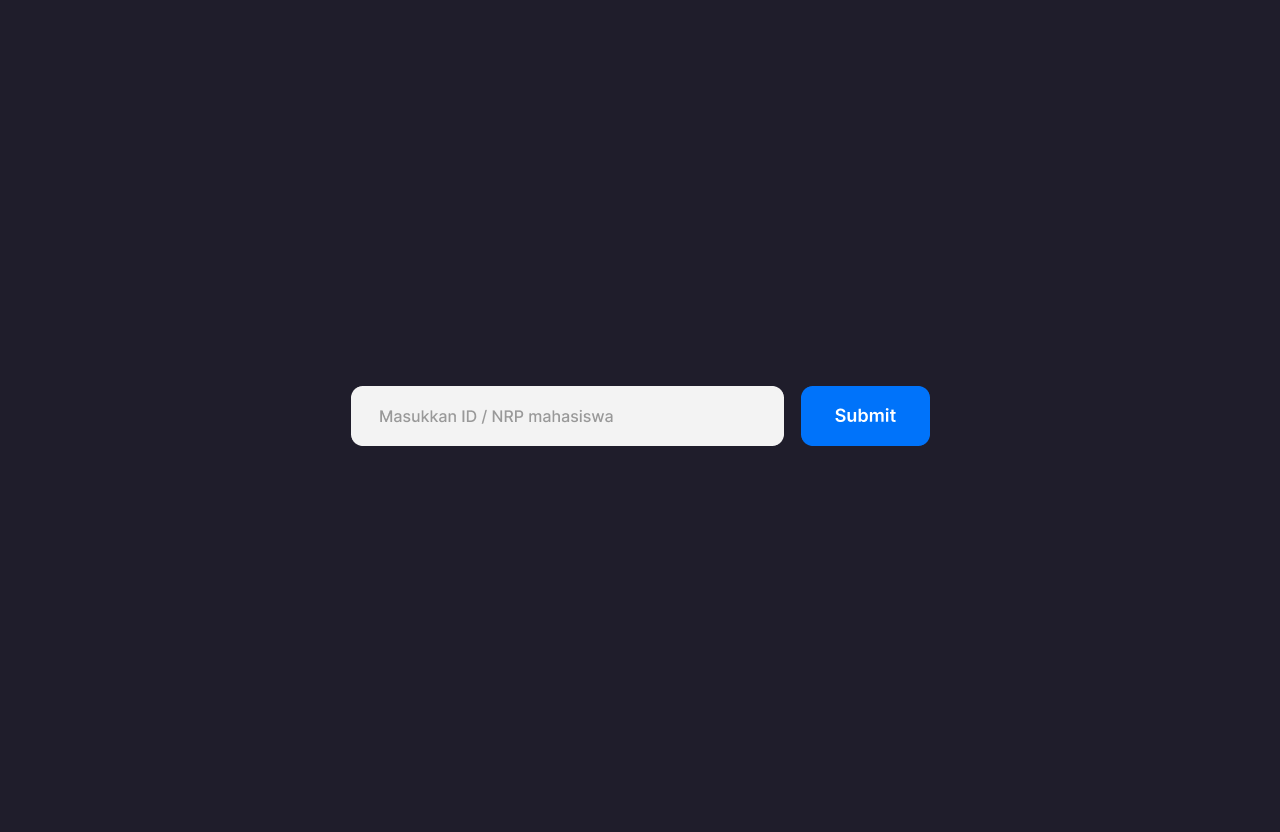
\includegraphics[width=150mm]{gambar/mockup-1.png}
    \vspace{2em}
    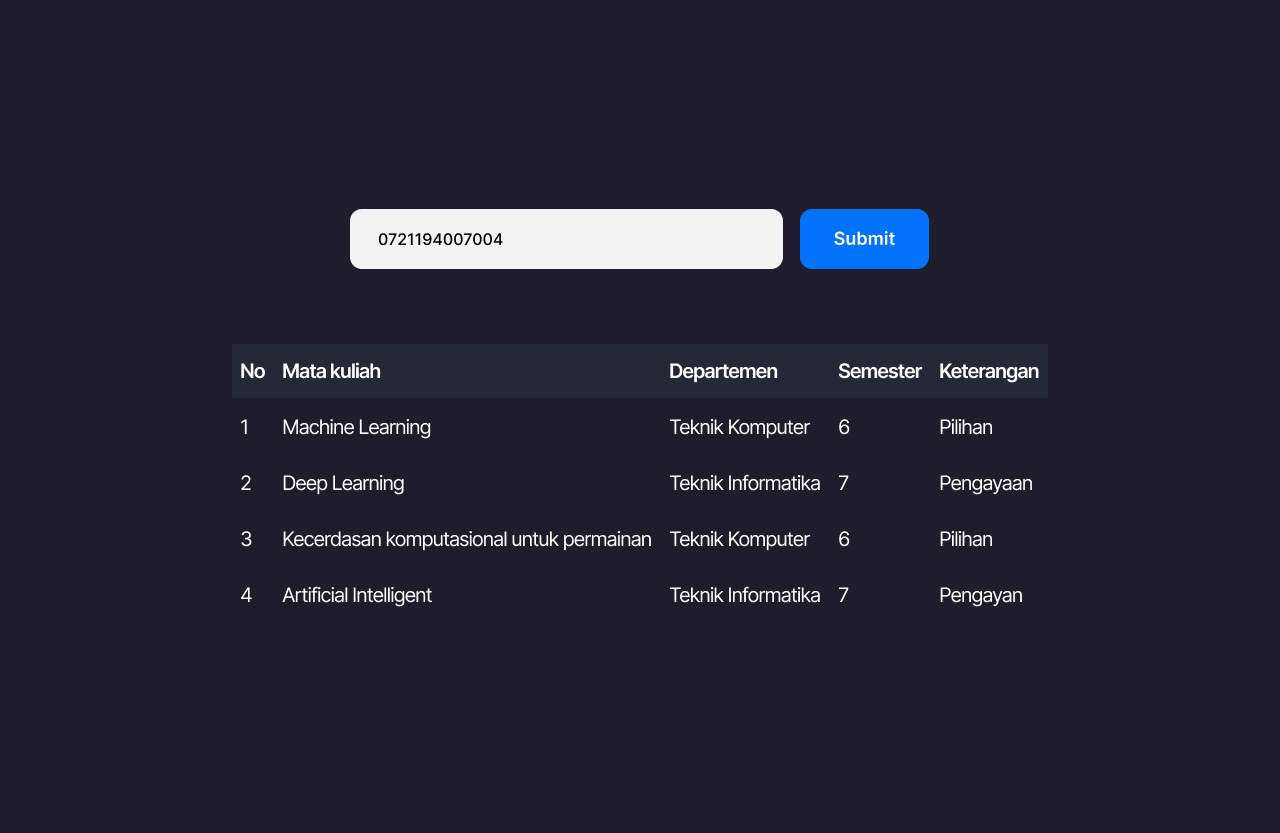
\includegraphics[width=150mm]{gambar/mockup-2.png}
    \caption{Mock Up Tampilan Website Sederhana}
  \end{figure}

\end{adjustwidth}





% Konten lainnya
% \chapter{HASIL YANG DIHARAPKAN}

\section{Hasil yang diharapkan dari penelitian}
Dari penelitian yang akan dilakukan, diharapkan dapat menghasilkan sebuah sistem yang mampu digunakan untuk
memberikan sebuah rekomendasi mata kuliah, sebagai alat bantu untuk mahasiswa dalam membuat keputusan. Dari penelitian ini juga
diharapkan pengembangan sistem rekomendasi ini dapat mempermudah mahasiswa menemukan mata kuliah yang sesuai minat dan kemampuan mereka,
khususnya mata kuliah pilihan dan mata kuliah pengayaan, sehingga dapat meminimalkan resiko mendapatkan nilai yang kurang memuaskan saat
menempuh mata kuliah yang dipilih akibat pemilihan mata kuliah yang tidak sesuai minat dan kemampuan.

\section{Hasil pendahuluan}
Sampai saat ini, kami telah melakukan eksplorasi mengenai struktur dataset yang umumnya digunakan untuk membuat sebuah sistem rekomendasi.
Selain itu, kami telah melakukan percobaan untuk membuat model sistem rekomendasi dengan pendekatan \emph{collaborative filtering}
dengan menggunakan dataset tersebut dan telah mencoba melakukan pembuatan \emph{API (Application Programming Interface)} agar rekomendasi yang
dihasilkan model sistem rekomendasi dapat diakses oleh aplikasi lain.

\newpage

\chapter*{JADWAL KEGIATAN}
\addcontentsline{toc}{chapter}{JADWAL KEGIATAN}
\newcommand{\w}{}
\newcommand{\G}{\cellcolor{gray}}
\begin{table}[h!]
    \begin{tabular}{|p{3.5cm}|c|c|c|c|c|c|c|c|c|c|c|c|c|c|c|c|}

        \hline
        \multirow{2}{*}{Kegiatan} & \multicolumn{16}{|c|}{Minggu}                                                                       \\
        \cline{2-17}              &
        1                         & 2                             & 3  & 4  & 5  & 6  & 7  & 8  & 9  & 10 & 11 & 12 & 13 & 14 & 15 & 16 \\
        \hline

        % Gunakan \G untuk mengisi sel dan \w untuk mengosongkan sel
        Pengumpulan data          &
        \G                        & \G                            & \G & \G & \w & \w & \w & \w & \w & \w & \w & \w & \w & \w & \w & \w \\
        \hline

        Analisa data              &
        \w                        & \w                            & \w & \w & \G & \G & \w & \w & \w & \w & \w & \w & \w & \w & \w & \w \\
        \hline

        Pengolahan data           &
        \w                        & \w                            & \w & \w & \w & \G & \G & \w & \w & \w & \w & \w & \w & \w & \w & \w \\
        \hline

        Pembuatan model           &
        \w                        & \w                            & \w & \w & \w & \w & \w & \G & \G & \G & \G & \w & \w & \w & \w & \w \\
        \hline

        Evaluasi model            &
        \w                        & \w                            & \w & \w & \w & \w & \w & \w & \w & \w & \G & \G & \G & \G & \w & \w \\
        \hline

        Deploy model              &
        \w                        & \w                            & \w & \w & \w & \w & \w & \w & \w & \w & \w & \w & \w & \G & \G & \w \\
        \hline

        Pembuatan web             &
        \w                        & \w                            & \w & \w & \w & \w & \w & \w & \w & \w & \w & \w & \w & \w & \G & \G \\
        \hline
    \end{tabular}
\end{table}

% Daftar pustaka
\section{DAFTAR PUSTAKA}
\renewcommand\refname{}
\bibliographystyle{unsrtnat}
\bibliography{pustaka/pustaka.bib}

\end{document}
